\FloatBarrier

\begin{figure}[h!]
	\centering
	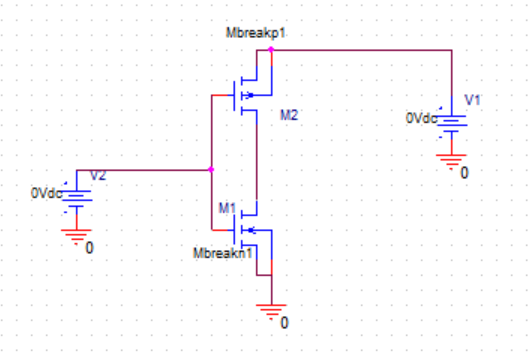
\includegraphics[scale=0.75]{./images/circuit1.PNG}
	\caption{CMOS Inverter Circuit}
	\label{fig:circuit1}
\end{figure}

\FloatBarrier

A DC sweep simulation is run to determine the voltage transfer characteristic for the CMOS inverter circuit in figure (\ref{fig:circuit1}).

\FloatBarrier

\begin{figure}[h!]
	\centering
	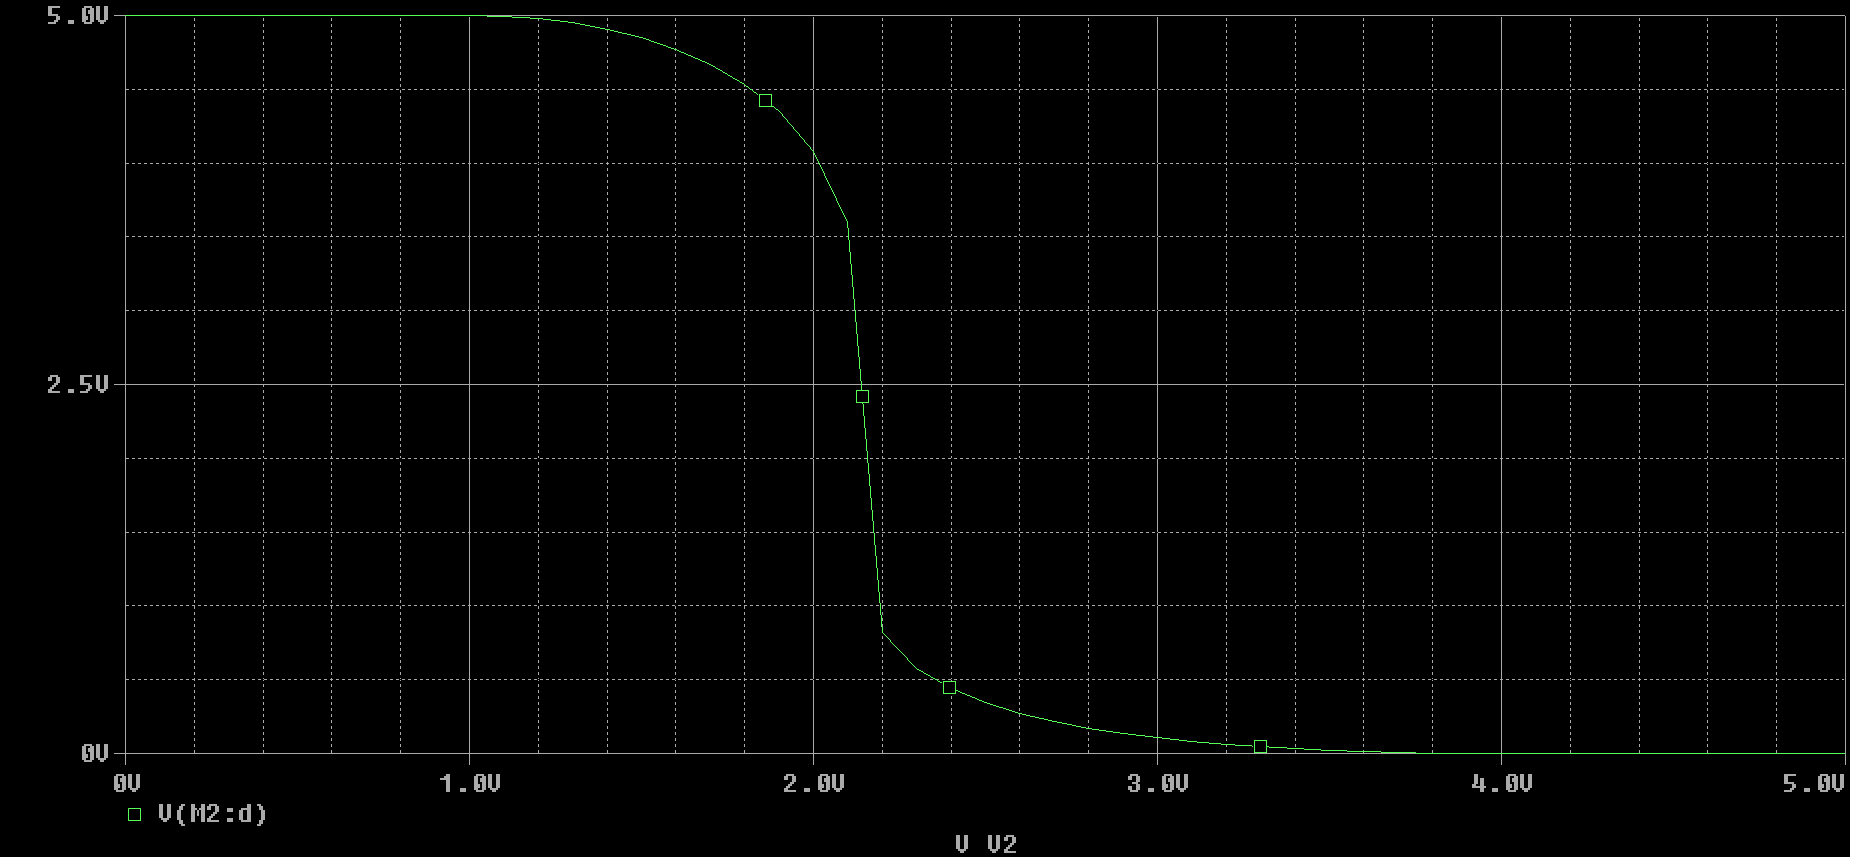
\includegraphics[scale=0.50]{./images/circuit1_dcsweep.PNG}
	\caption{Figure (\ref{fig:circuit1}) Circuit Voltage Transfer Characteristic}
	\label{fig:circuit1_dcsweep}
\end{figure}

\FloatBarrier

At low input gate voltages, "low" meaning "close to ground", $V_{GS}$ for the NMOS on the bottom drops below its threshold voltage. Therefore, no current flows through the NMOS transistor. However, $V_{SG}$ for the PMOS on the top exceeds its threshold voltage. As a result, the PMOS transistor is on and sets the output voltage to the supply voltage. If a load capacitance is connected to the output of the inverter, it is charged to the supply voltage, in this case $5$\si{\volt}. \\

At high input gate voltages, "high" meaning "close to supply", $V_{GS}$ for the NMOS exceeds its threshold voltage, and the output voltage node is grounded. However, the PMOS is turned off since the input gate voltage is close to its source voltage. Because the output voltage is high when the input voltage is low and the output voltage is low when the input voltage is high, the circuit essentially "inverts" the input, hence the name "inverter". Assuming the output voltage is a continuous function of the input voltage, the CMOS inverter gradually moves from supply to ground as the input gate voltage is increased. \\

\FloatBarrier

\begin{figure}[h!]
	\centering
	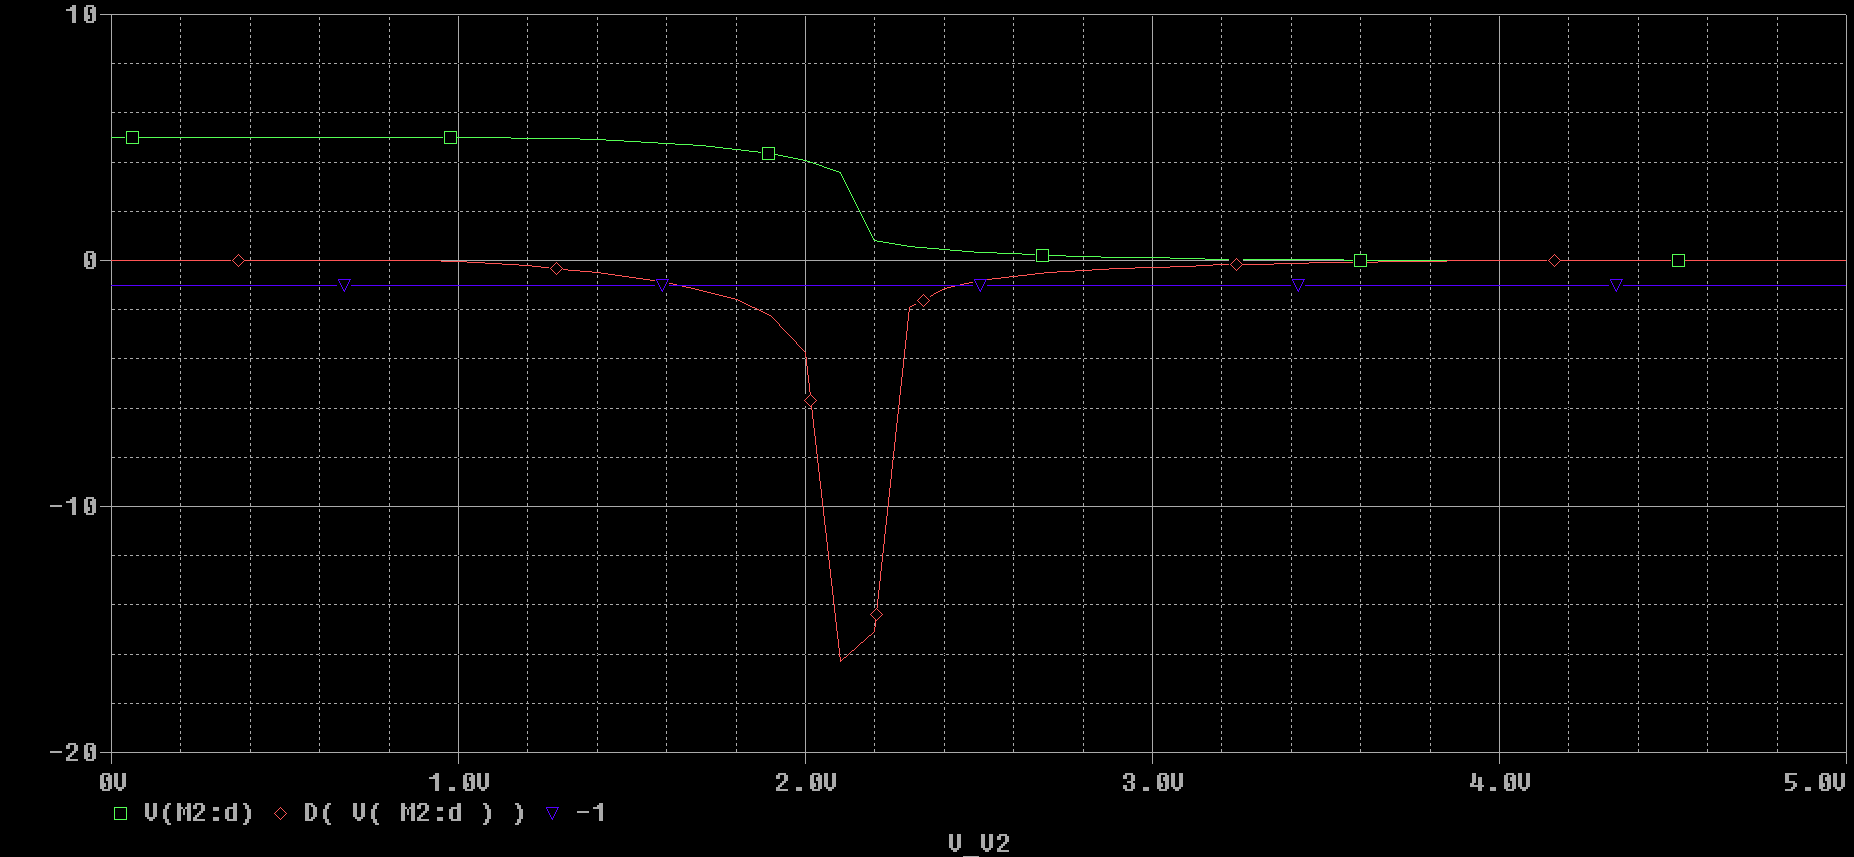
\includegraphics[scale=0.50]{./images/circuit1_noisemargin_measure.PNG}
	\caption{CMOS Inverter Noise Margin Measurement}
	\label{fig:circuit1_noisemargin_measure}
\end{figure}

\FloatBarrier

{\footnotesize The green curve is the voltage transfer characteristic. The red curve is $\frac{dV_{out}}{dV_{in}}$. The blue line is simply the value $-1$. The x-coordinate of the first point of intersection of the red and blue lines is $V_{IL}$. The x-coordinate of the second intersection is $V_{IH}$.}

\FloatBarrier

The noise margins $NM_{L}$ and $NM_{H}$ for the CMOS inverter can be acquired from analyzing its voltage transfer characteristic (VTC). Let $V_{IL}$ be the point at which the slope of the VTC curve is $-1$ when the NMOS is turned off. $V_{IL}$ is the highest value of input gate voltage such that the output can be correctly interpreted as a "1", or high voltage level. Past that point, the circuit no longer operates as an inverter and begins to act more as a voltage amplifier. Similarly, let $V_{IH}$ be the point at which the slope is $-1$ when the PMOS is turned off. $V_{IH}$ is the minimum gate input voltage such that the output is correctly interpreted as a "0". $V_{OH}$ is the inverter's output voltage when the input voltage is grounded. $V_{OL}$ is the output when the input is set to supply. The noise margins are then defined by the following equations:

\begin{equation}
	\label{eq:nml}
	NM_{L} = V_{IL} - V_{OL}
\end{equation}

\begin{equation}
	\label{eq:nmh}
	NM_{H} = V_{OH} - V_{OL}
\end{equation}

Regarding equations (\ref{eq:nml}) and (\ref{eq:nmh}), $NM_{L}$ and $NM_{H}$ are the largest voltage levels of noise that can be introduced to the inverter's output before its logic level is incorrect. $V_{OL}$ and $V_{OH}$ are clearly $0$\si{\volt} and $5$\si{\volt} from the VTC curve. $V_{IH}$ and $V_{IL}$ can be determined by analyzing the points at which the slope of the VTC is $-1$. This is what figure (\ref{fig:circuit1_noisemargin_measure}) depicts. So, $V_{IL} = 1.6340$\si{\volt}, and $V_{IH} = 2.4438$\si{\volt}. Therefore, the noise margins are given by $NM_{L} = 1.6340$\si{\volt} and $NM_{H} = 2.5562$\si{\volt}. \\

\FloatBarrier

\begin{figure}[h!]
	\centering
	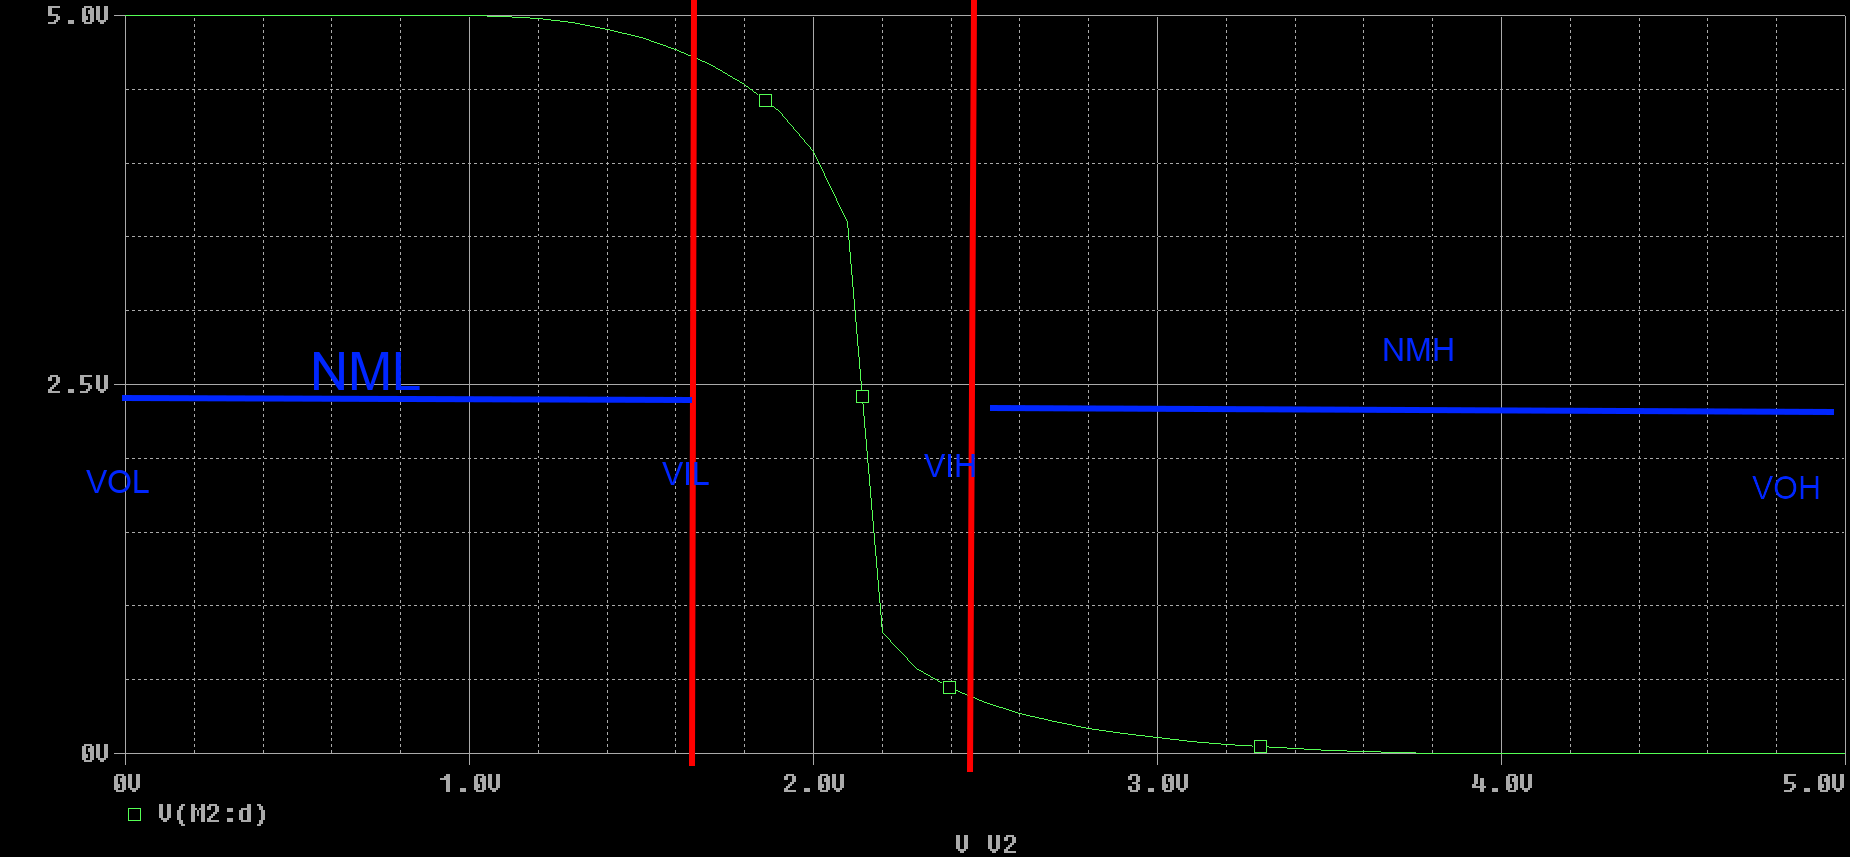
\includegraphics[scale=0.25]{./images/circuit1_noisemargin.PNG}
	\caption{Depiction of Noise Margins on Voltage Transfer Characteristic}
	\label{fig:circuit1_noisemargin}
\end{figure}

\FloatBarrier

The CMOS inverter, unlike other inverters like common-source amplifiers, is designed for optimal noise margins. For other inverters, $V_{OH}$ and $V_{OL}$ do not fully reach supply and ground respectively. In the case of a common-source amplifier, when the input voltage is close to supply, the transistor operates in the triode mode. Therefore, the circuit operates like a voltage divider, and the output voltage does not fully reach ground. As a result, a lower noise voltage is required to flip an output "0" to the amplifier state or even a "1". However, in a CMOS inverter, one of the transistors is in cutoff when the output is a "1" or a "0". Therefore, the open circuit fully consumes the supply voltage, meaning the output voltage hits either supply or ground. Thus, it takes a higher noise voltage to cause the inverter's output to be incorrect. \\

\FloatBarrier

\begin{figure}[h!]
	\centering
	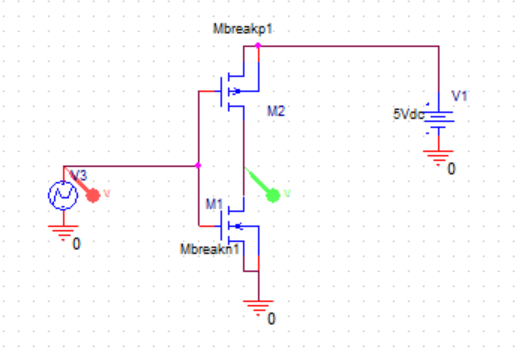
\includegraphics[scale=0.75]{./images/circuit2.PNG}
	\caption{CMOS Inverter with Square-Wave Input}
	\label{fig:circuit2}
\end{figure}

\FloatBarrier

The circuit in figure (\ref{fig:circuit2}) is used to observe the inverter's transient behavior.

\FloatBarrier

\begin{figure}[h!]
	\centering
	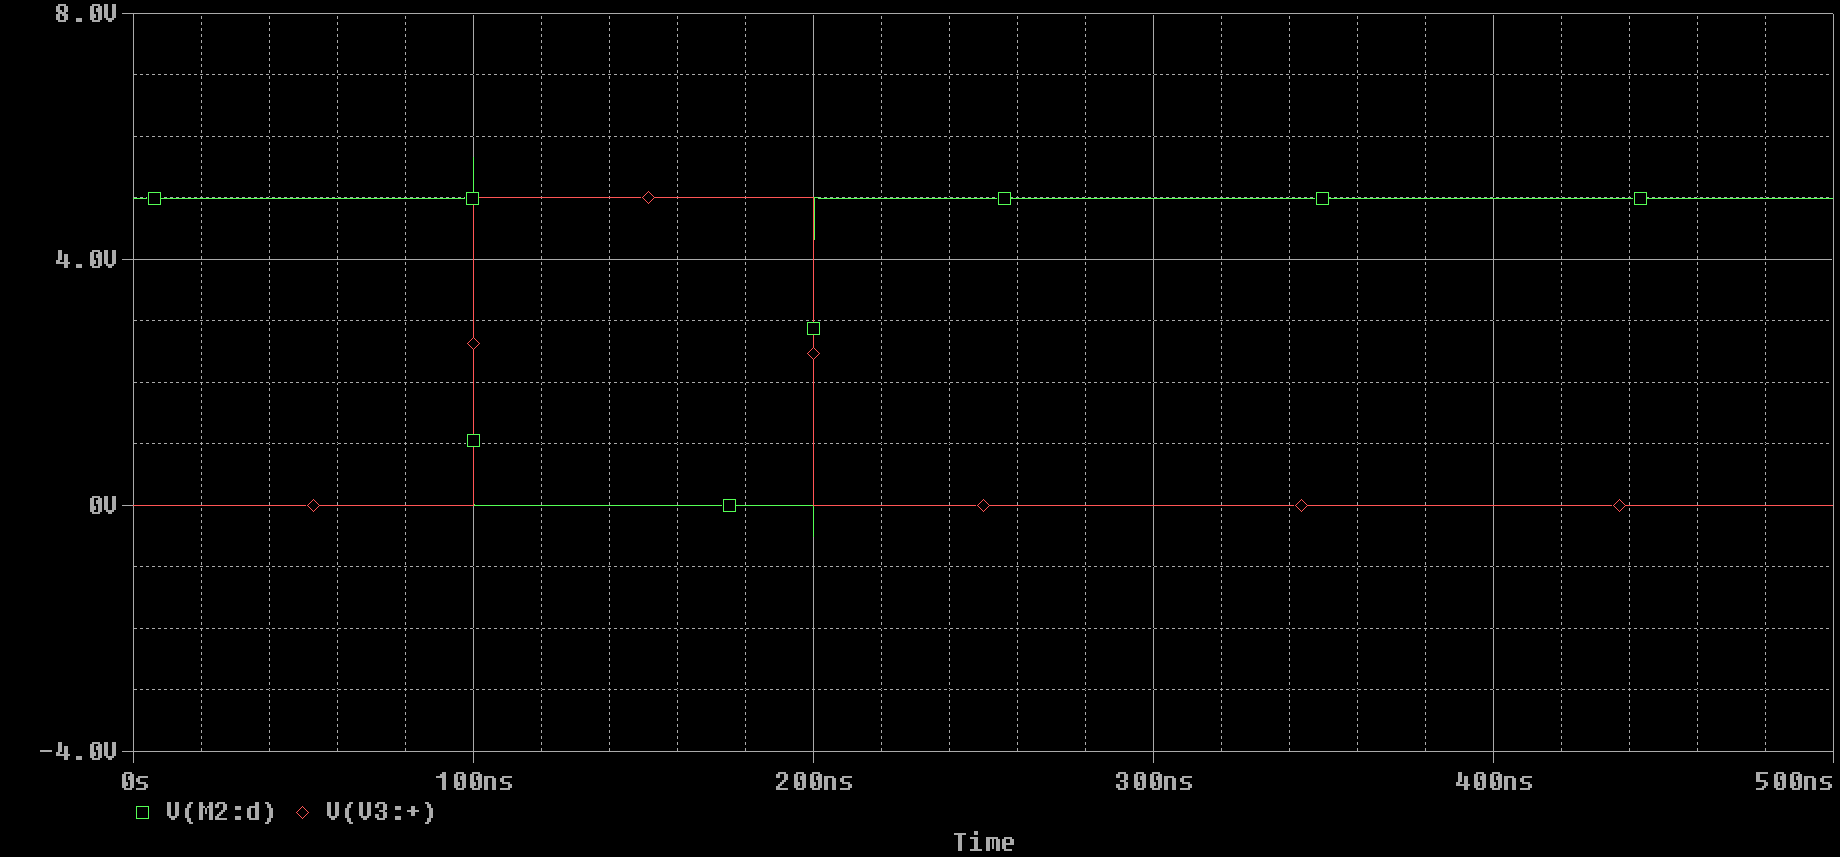
\includegraphics[scale=0.65]{./images/circuit2_transient.PNG}
	\caption{Transient Analysis of the Circuit in Figure (\ref{fig:circuit2})}
	\label{fig:circuit2_transient}
\end{figure}

\FloatBarrier

{\footnotesize The green curve is the output voltage, and the red curve is the input voltage.}

\FloatBarrier

The propagation delay can be ascertained from the transient response in figure (\ref{fig:circuit2_transient}). $t_{PLH}$ is defined as the time it takes for the inverter's output to transition from half the supply voltage to the supply voltage. $t_{PHL}$ is the time it takes the inverter to transition from the supply voltage to half the supply voltage. The propagation delay is therefore defined by the following equation:
 
\begin{equation}
	\label{eq:prop_delay}
	t_{p} = \frac{t_{PHL} + t_{PLH}}{2}
\end{equation}

Because $t_{PHL} = 81$\si{\pico\second} and $t_{PLH} = 103$\si{\pico\second}, the propagation delay $t_p = 92$\si{\pico\second}.
